% Bone — a skull sitting straight on the ribs, with nothing between them. The
% first draft drew the two apart and the ribs came out as a spring; they are
% one silhouette now, which is what a ribcage is.
%
% Written by filling in tikz_figure_prompt.md.
\documentclass[tikz,border=4pt]{standalone}
\usetikzlibrary{calc}
\providecommand{\Main}{DFDCCF}
\providecommand{\Dark}{9C9787}
\providecommand{\Accent}{8B4225}

\newcommand{\Unit}{0.055cm}
\newcommand{\Edge}{2.0pt}
\newcommand{\Ribs}{4}
\newcommand{\RibW}{19}         % half-width of the widest rib

\definecolor{main}{HTML}{\Main}
\definecolor{dark}{HTML}{\Dark}
\definecolor{accent}{HTML}{\Accent}
\definecolor{ink}{HTML}{101018}

\begin{document}
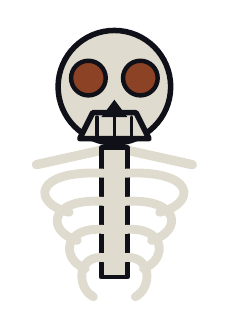
\begin{tikzpicture}[x=\Unit,y=\Unit, line join=round, line cap=round]

  % ---- collarbones, which carry the skull and close the top of the cage ---
  \draw[main,line width=3.4pt] (32,36) -- (14,32);
  \draw[main,line width=3.4pt] (32,36) -- (50,32);

  % ---- sternum ------------------------------------------------------------
  \fill[main,draw=ink,line width=1.6pt] (29,6) rectangle (35,36);

  % ---- ribs: widest at the top, tapering down, so the cage is a cage ------
  \foreach \i in {1,...,\Ribs} {
    \pgfmathsetmacro\y{30-(\i-1)*6.5}
    \pgfmathsetmacro\w{\RibW-(\i-1)*3.4}
    \draw[main,line width=3.2pt]
      (30,\y) .. controls ({32-\w},\y+1) and ({32-\w},{\y-7}) .. ({32-\w*0.55},{\y-9});
    \draw[main,line width=3.2pt]
      (34,\y) .. controls ({32+\w},\y+1) and ({32+\w},{\y-7}) .. ({32+\w*0.55},{\y-9});
  }

  % ---- skull, sitting on the collarbones ---------------------------------
  \fill[main,draw=ink,line width=\Edge] (32,50) circle (13);
  % Jaw: one piece, tucked under the cranium rather than hung below it.
  \fill[main,draw=ink,line width=\Edge] (24,38) -- (40,38) -- (37,44) -- (27,44) -- cycle;
  \foreach \x in {28,32,36} { \draw[ink,line width=1.2pt] (\x,38.5) -- (\x,43); }

  % ---- sockets: the accent, and the only saturated thing on the figure ----
  \fill[accent,draw=ink,line width=1.6pt] (26,52) circle (4.0);
  \fill[accent,draw=ink,line width=1.6pt] (38,52) circle (4.0);
  \fill[ink] (32,47) -- (29,43) -- (35,43) -- cycle;   % nasal

\end{tikzpicture}
\end{document}
